%==============================================================================%
%                PRØVE | FORKURS 1P-2P LÆRERUTDANNING | V2016                  %
%==============================================================================%
%
% __/\\\\\\\\\\\\____________________/\\\\\\______________/\\\\\\\\\_____
%  _\/\\\////////\\\_________________\////\\\____________/\\\///////\\\___
%   _\/\\\______\//\\\___________________\/\\\___________\///______\//\\\__
%    _\/\\\_______\/\\\_____/\\\\\\\\_____\/\\\_____________________/\\\/___
%     _\/\\\_______\/\\\___/\\\/////\\\____\/\\\__________________/\\\//_____
%      _\/\\\_______\/\\\__/\\\\\\\\\\\_____\/\\\_______________/\\\//________
%       _\/\\\_______/\\\__\//\\///////______\/\\\_____________/\\\/___________
%        _\/\\\\\\\\\\\\/____\//\\\\\\\\\\__/\\\\\\\\\_________/\\\\\\\\\\\\\\\_
%         _\////////////_______\//////////__\/////////_________\///////////////_
%
%==============================================================================%
%                               MED HJELPEMIDLER                               %
%==============================================================================%

\Del{m}


%==============================================================================%
%                                 OPPGAVE 2.1                                  %
%==============================================================================%
\Oppgave[1] \points*{1}

Skyskraperen Burj Khalifa i Dubai er $\SI{828}{\m}$ høy. Et kronestykke er
$\SI{1.7}{\mm}$ tykt. Tenk deg at du skal bygge et tårn av kronestykker. Tårnet
skal være like høyt som Burj Khalifa. \bigskip

Omtrent hvor mange kronestykker vil du trenge? Skriv svaret på standardform.


%==============================================================================%
%                                 OPPGAVE 2.2                                  %
%==============================================================================%
\Oppgave[7]

En bedrift vil starte produksjon av et nytt produkt. Anta at funksjonen $f$ er
gitt ved
%
\begin{equation*}
  f(x)
  = \num{9.2} x^3 - 880x^2 + \num{22000} x \ ,
  \qquad 0 \leq x \leq 36
\end{equation*}
%
kan brukes som modell for hvor mange enheter $f(x)$ av produktet bedriften vil
kunne selge $x$ måneder etter produksjonsstart.

\begin{oppgaver}
  \Item{1} Bruk graftegner til å tegne grafen $f$.
\end{oppgaver}

\begin{oppgaver}
  \Item{2} I hvor mange måneder vil bedriften kunne selge over $\num{100000}$
    enheter ifølge modellen?
\end{oppgaver}

\begin{oppgaver}
  \Item{2} Bestem gjennomsnittlig vekstfart fra $x = 2$ til $x = 10$. Hvilken
    praktisk informasjon gir dette svaret?
\end{oppgaver}

\begin{oppgaver}
  \Item{2} Bestem den momentane vekstfarten for $x = 25$. Hvilken praktisk
    informasjon gir dette svaret?
\end{oppgaver}


%==============================================================================%
%                                 OPPGAVE 2.3                                  %
%==============================================================================%
\Oppgave[4]

Antall individer av en dyreart i et området har avtatt siden $1970$. Se

\begin{table}[H]
  \newcommand{\tbnum}[1]{\multirow{-2}{*}{$\num{#1}$}}
    \centering
    \caption{}
    \label{tab:del-1-oppgave-1.4}
    \begin{tabularx}{\textwidth}{| l | *{5}{Y|} } \hline
      \Cellcolor{År}        &    $1970$     &    $1980$     &    $1990$     &    $2000$    &    $2010$ \\ \hline
      \Cellcolor{Antall}    &               &               &               &              & \\[-0.02cm]
      \Cellcolor{individer} & \tbnum{40000} & \tbnum{24100} & \tbnum{14600} & \tbnum{8400} & \tbnum{5100} \\
        \hline
    \end{tabularx}
\end{table}

\begin{oppgaver}
  \Item{2} Bruk regresjon til å bestemme en eksponentiell modell som viser
    antall individer av dyrearten i området $x$ år etter $1970$.
    \label{delopg:del-1-oppgave-2.3a}
\end{oppgaver}

\begin{oppgaver}
  \Item{1} Hvor mange prosent avtar antall individer med per år i følge
    modellen i \cref{delopg:del-1-oppgave-2.3a}.
\end{oppgaver}

\begin{oppgaver}
  \Item{1} Når vil det være $\num{1000}$ individer av dyrearten i området
    ifølge modellen i \cref{delopg:del-1-oppgave-2.3a}?
\end{oppgaver}


%==============================================================================%
%                                 OPPGAVE 2.4                                  %
%==============================================================================%
\Oppgave[2] \points*{2}

I en klasse er det $20$ elever. $10$ av elevene har eldre søsken, $15$ har yngre
søsken, $2$ av elevene har ikke søsken. \bigskip

Tenk deg at du skal trekke èn elev fra klassen tilfeldig \bigskip

Bestem sannsynligheten for at du komme til å trekke en elev som har eldre, men
ikke yngre, søsken.


%==============================================================================%
%                                 OPPGAVE 2.5                                  %
%==============================================================================%
\Oppgave[3] \points*{3}

\begin{figure}[H]
  \centering
  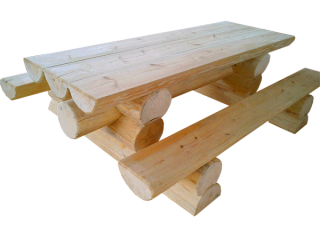
\includegraphics[width=0.5\linewidth]{picnic.png}
  \caption{}
  \label{fig:del-2-oppgave-2.5a}
\end{figure}

Tenk deg at du skal lage et bord av tømmerstokker som vist i
\cref{fig:del-2-oppgave-2.5a}. \bigskip

Bordplaten skal bestå av tre halve tømmerstokker. Disse stokkene skal være
$\SI{2.5}{\m}$ lange. Anta at tverrsnittet til hver halve tømmerstokk har form
som en halvsirkel med diameter $\SI{30}{\cm}$. Se \cref{fig:del-2-oppgave-2.5b}.


\begin{figure}[H]
  \centering
  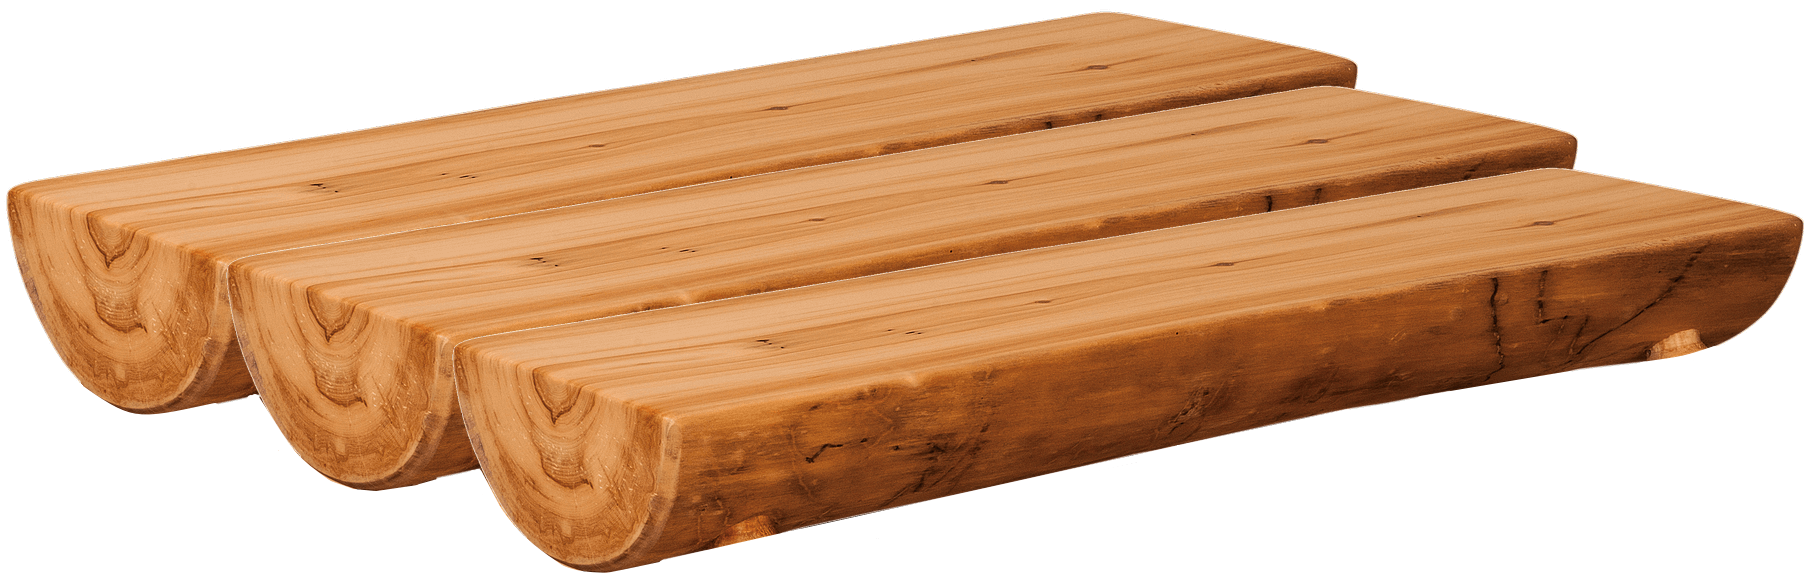
\includegraphics[width=0.5\linewidth]{threeLogs.png}
  \caption{}
  \label{fig:del-2-oppgave-2.5b}
\end{figure}

Før du setter sammen bordet, skal hele overflaten til hver av disse tre halve
stokkene lakkeres. \bigskip

Hvor mange desiliter lakk trenger du når $\SI{1}{\L}$ lakk er nok til
$\SI{10}{\m\squared}$?


%==============================================================================%
%                                 OPPGAVE 2.6                                  %
%==============================================================================%
\Oppgave[4]

\begin{table}[H]
    \centering
    \caption{}
    \label{tab:del-2-oppgave-2.6}
    \begin{tabular}{|l |S[table-format=3.0]|} \hline
      \Rowcolor & {Treningstid}\\[-0.02cm] \Rowcolor
         \multirow{-2}{*}{Dag} & {(minutter)}  \\ \hline
         Mandag  &  60 \\ \hline
         Tirsdag &  90 \\ \hline
         Onsdag  &  60 \\ \hline
         Torsdag &  80 \\ \hline
         Fredag  &  75 \\ \hline
         Lørdag  &  60 \\ \hline
         Mandag  & 100 \\ \hline
    \end{tabular}
\end{table}

\cref{tab:del-2-oppgave-2.6} ovenfor viser hvor mange minutter Kristian trente i
forrige uke.

\begin{oppgaver}
  \Item{1} Hvor mange minutter trente Kristian i gjennomsnitt per dag?
\end{oppgaver}

\begin{oppgaver}
  \Item{1} Bestem standardavviket for treningstidene.
\end{oppgaver}

Du får vite følgende om Ståle:

\begin{itemize}
  \item Han trente også hver dag forrige uke.
  \item{I gjennomsnitt trente han like mange minutter som Kristian per dag}
  \item Treningstidene hans har høyere standardavvik enn treningstidene til
    Kristian.
\end{itemize}

\begin{oppgaver}
  \Item{2} Sett opp en tabell som viser hvor mange minutter Ståle \emph{kan}
    ha trengt hver dag i forrige uke ut i fra opplysningene ovenfor. Forklar
    hvordan du har tenkt.
\end{oppgaver}


%==============================================================================%
%                                 OPPGAVE 2.7                                  %
%==============================================================================%
\Oppgave[8]

Arbeidstakere må betale $\SI{25}{\percent}$ skatt av alminnelig inntekt* og
$\SI{8.2}{\percent}$ trygdeavgift av personinntekt.

Arbeidstakere som har personinntekt over $\num{159800}$ kroner, må i tillegg
betale trinnskatt. Trinnskatten består av fire trinn og beregnes slik:

\begin{itemize}
  \item $\SI{0.44}{\percent}$ av den delen av personinntekten som er mellom
    $\num{159800}$ og $\num{224900}$~kroner.
  \item $\SI{1.7}{\percent}$ av den delen av personinntekten som er mellom
    $\num{224900}$ og $\num{565400}$~kroner.
  \item $\SI{10.7}{\percent}$ av den delen av personinntekten som er mellom
    $\num{565400}$ og $\num{909500}$~kroner.
  \item $\SI{13.7}{\percent}$ av den delen av personinntekten som er over
    $\num{909500}$~kroner.
\end{itemize}

\begin{table}[hbp!]
  \centering\small
  \setlength{\extrarowheight}{1pt}
  \caption{}
  \label{tab:del-2-oppgave-2.7}
  \begin{adjustbox}{center}
    \begin{tabular}{|l|l|l|l|r|r|r|}

      \hhline{*{7}{-}}
      \dgr{}
    &\mcdg{A}
    & \mcdg{B}
    &\mcdg{C}
    &\mcdg{D}
    &\mcdg{E}
    &\mcdg{F}
    \\
    \hhline{*{7}{-}}
    \midg{1}
    &\mig{}
    &\tableTitle
    \\
    \hhline{|-|*{6}{>{\arrayrulecolor{lightGray}}-}|}\arrayrulecolor{black}
    \midg{2}
    &\blvi{}
    \\
    \hhline{|-|>{\arrayrulecolor{lightGray}}->{\arrayrulecolor{black}}--|>{\arrayrulecolor{lightGray}}---|}
    \arrayrulecolor{black}
    \midg{3}
    &\lgr
    &\dgr\textbf{Personinntekt:}
    &% white cell
    &\bliii
    \\
    \hhline{|-|>{\arrayrulecolor{lightGray}}->{\arrayrulecolor{black}}--|>{\arrayrulecolor{lightGray}}---|}
    \arrayrulecolor{black}
    \midg{4}
    &\lgr
    &\dgr\textbf{Samlet fradrag:}
    &% white cell
    &\bliii
    \\
    \hhline{|-|>{\arrayrulecolor{lightGray}}->{\arrayrulecolor{black}}--|>{\arrayrulecolor{lightGray}}---|}
    \arrayrulecolor{black}
    \midg{5}
    &\lgr
    &\dgr\textbf{Alminnelig inntekt:}
    &\cellcolor{maincolorLight}
    &\bliii
    \\
    \hhline{|-|>{\arrayrulecolor{lightGray}}->{\arrayrulecolor{black}}--|>{\arrayrulecolor{lightGray}}---|}
    \arrayrulecolor{black}
    \midg{6}
    &\blvi{}
    \\
    \hhline{|-|*{6}{>{\arrayrulecolor{lightGray}}-}|}
    \arrayrulecolor{black}
    \midg{7}
    &\blvi{}
    \\
    \hhline{|-|>{\arrayrulecolor{lightGray}}->{\arrayrulecolor{black}}---|>{\arrayrulecolor{lightGray}}--|}
    \arrayrulecolor{black}
    \midg{8}
    &\lgr
    &\dgr \textbf{Skatt}
    &\dgr\textbf{Prosentsats}
    &\dgr\textbf{Beløp}
    &\blii
    \\
    \hhline{|-|>{\arrayrulecolor{lightGray}}->{\arrayrulecolor{black}}---|>{\arrayrulecolor{lightGray}}--|}
    \arrayrulecolor{black}
    \midg{9}
    &\lgr
    &\dgr\textbf{alminnelig inntekt:}
    &\mcdg{25\,\%}
    &\cellcolor{maincolorLight}
    &\blii
    \\
    \hhline{|-|>{\arrayrulecolor{lightGray}}->{\arrayrulecolor{black}}---|>{\arrayrulecolor{lightGray}}--|}
    \arrayrulecolor{black}
    \midg{10}
    &\lgr
    &\dgr\textbf{Trygdeavgift:}
    &\mcdg{8,5\,\%}
    &\cellcolor{maincolorLight}
    &\blii
    \\
    \hhline{|-|>{\arrayrulecolor{lightGray}}->{\arrayrulecolor{black}}---|>{\arrayrulecolor{lightGray}}--|}
    \arrayrulecolor{black}
    \midg{11}
    &\blvi{}
    \\
    \hhline{|-|*{6}{>{\arrayrulecolor{lightGray}}-}|}
    \arrayrulecolor{black}
    \midg{12}
    &\mig{}
    &\blv{\textbf{Trinnskatt}}
    \\
    \hhline{|-|>{\arrayrulecolor{lightGray}}->{\arrayrulecolor{black}}-----|}
    \midg{13}
    &\lgr
    &\dgr
    &\dgr{\textbf{Prosentsats}}
    &\mcdg{\textbf{Fra}}
    &\mcdg{\textbf{Til}}
    &\dgr{\textbf{Trinnskatt}}
    \\
    \hhline{|-|>{\arrayrulecolor{lightGray}}->{\arrayrulecolor{black}}-----|}
    \midg{14}
    &\lgr
    &\dgr\textbf{Trinn 1:}
    &\mcdg{0,44\,\%}
    &\dgr{159\,800,00}
    &\dgr{224\,900,00}
    &\cellcolor{maincolorLight}\textbf{286,44}
    \\
    \hhline{|-|>{\arrayrulecolor{lightGray}}->{\arrayrulecolor{black}}-----|}
    \midg{15}
    &\lgr
    &\dgr\textbf{Trinn 2:}
    &\mcdg{1,7\,\%}
    &\dgr{224\,900,00}
    &\dgr{565\,400,00}
    &\cellcolor{maincolorLight}\textbf{5788,50}
    \\
    \hhline{|-|>{\arrayrulecolor{lightGray}}->{\arrayrulecolor{black}}-----|}
    \midg{16}
    &\lgr
    &\dgr\textbf{Trinn 3:}
    &\mcdg{10,7\,\%}
    &\dgr{565\,400,00}
    &\dgr{909\,500,00}
    &\cellcolor{maincolorLight}
    \\
    \hhline{|-|>{\arrayrulecolor{lightGray}}->{\arrayrulecolor{black}}-----|}
    \midg{17}
    &\lgr
    &\dgr\textbf{Trinn 4:}
    &\mcdg{13,7\,\%}
    &\dgr{909\,500,00}
    &\dgr
    &\cellcolor{maincolorLight}
    \\
    \hhline{|-|>{\arrayrulecolor{lightGray}}->{\arrayrulecolor{black}}-----|}
    \midg{18}
    &\lgr
    &\dgr\textbf{Totalt:}
    &\dgr
    &\dgr
    &\dgr
    &\cellcolor{maincolorLight}
    \\
    \hhline{|-|>{\arrayrulecolor{lightGray}}->{\arrayrulecolor{black}}-----|}
    \midg{19}
    &\blvi{}
    \\
    \hhline{|-|>{\arrayrulecolor{lightGray}}->{\arrayrulecolor{black}}--|>{\arrayrulecolor{lightGray}}---|}
    \arrayrulecolor{black}
    \midg{20}
    &\lgr
    &\dgr\textbf{Samlet skatt:}
    &\cellcolor{maincolorLight}
    &\bliii
    \\
    \hhline{|-|>{\arrayrulecolor{lightGray}}->{\arrayrulecolor{black}}--|>{\arrayrulecolor{lightGray}}---|}
    \arrayrulecolor{black}
    \midg{21}
    &\blvi{}
    \\
    \lasthline
    \end{tabular}
  \end{adjustbox}
\end{table}

I \cref{tab:del-2-oppgave-2.7} ser du et regneark for enkel skatteberegning for
arbeidstakere med personinntekt over $\num{565400}$ kroner på grunnlag av
opplysningene ovenfor.

\begin{oppgaver}
  \Item{2} Vis at beløpene i cellene F$14$ og F$15$ alltid vil bli
    $\num{286.44}$ og $\num{5788.50}$ for arbeidstakere med personinntekt over
    $\num{565400}$ kroner.
\end{oppgaver}

Ola har en personinntekt på $\num{666000}$ kroner og et samlet fradag på
$\num{154100}$ kroner. Kari har en personinntekt på $\num{1114000}$ kroner og
et samlet fradag på $\num{184500}$ kroner.

\begin{oppgaver}
  \Item{5} Du skal lage et regneark som både Ola og Kari kan bruke til å
    beregne samlet skatt. Lag regnearket som vist ovenfor. Ola og Kari skal
    kunne legge inn personinntekt og fradrag i de hvite cellene. I de fargelagte
    cellene skal du sette inn formler. Vis hvilke formler du har brukt.
\end{oppgaver}

\begin{oppgaver}
  \Item{1} Bruk regnearket og beregn samlet skatt for Ola og samlet skatt for
    Kari.
\end{oppgaver}


%==============================================================================%
%                                 OPPGAVE 2.8                                  %
%==============================================================================%
\Oppgave[7]

\begin{figure}[H]
  \centering
  \begin{subfigure}[b]{0.25\textwidth}
    \centering
    \tikzsetnextfilename{Forkurs-1p-2p-laererutdanning-2016-V-oppgave-2-8a}
    \drawTetris{1}
    \caption{}
    \label{fig:del-1-oppgave-8-a}
  \end{subfigure}\hfill%
  \begin{subfigure}[b]{0.32\textwidth}
    \centering
    \tikzsetnextfilename{Forkurs-1p-2p-laererutdanning-2016-V-oppgave-2-8b}
    \drawTetris{2}\vspace*{-0.5cm}
    \caption{}
    \label{fig:del-1-oppgave-8-b}
  \end{subfigure}\hfill%
  \begin{subfigure}[b]{0.41\textwidth}
    \centering
    \tikzsetnextfilename{Forkurs-1p-2p-laererutdanning-2016-V-oppgave-2-8c}
    \drawTetris{3}
    \caption{}
    \label{fig:del-1-oppgave-8-c}
  \end{subfigure}
  \caption{}\label{fig:del-1-oppgave-8}
\end{figure}

I \cref{fig:del-1-oppgave-8} ser du de tre første figurene i en serie som kan
fortsettes. Figurene er sammen av hvite og fargede kvadrater.

\begin{oppgaver}
  \Item{1} Bestem antall grå og antall lilla kvadrater i (4)
\end{oppgaver}

\begin{oppgaver}
  \Item{2} Bestem et uttrykk for antall hvite kvadrater i figur $(n)$ uttrykt
    ved $n$.
\end{oppgaver}

\begin{oppgaver}
  \Item{2} Bestem et uttrykk for antall lilla kvadrater i figur $(n)$ uttrykt
    ved $n$.
\end{oppgaver}

Tenk deg at du har $\num{1000}$ hvite og $\num{1200}$ fargede kvadrater. Du skal
lage en figur eter samme mønster som ovenfor. Figuren skal være så stor som
mulig.

\begin{oppgaver}
  \Item{2} Hvor mange kvadrater vil denne figuren inneholde totalt?
\end{oppgaver}
